\documentclass[12pt]{article}
\usepackage{graphicx}
\usepackage{amsmath}
\usepackage{hyperref}
\usepackage{listings}
\usepackage{color}
\usepackage[a4paper, total={6in, 8in}]{geometry}

\usepackage{changepage}
\usepackage{booktabs}

\graphicspath{ {images/} }


% Define colors for code listings
\definecolor{codegray}{rgb}{0.5,0.5,0.5}
\definecolor{codepurple}{rgb}{0.58,0,0.82}
\definecolor{backcolour}{rgb}{0.95,0.95,0.92}

\lstdefinestyle{mystyle}{
    backgroundcolor=\color{backcolour},
    commentstyle=\color{codegray},
    keywordstyle=\color{blue},
    numberstyle=\tiny\color{codegray},
    stringstyle=\color{codepurple},
    basicstyle=\ttfamily\footnotesize,
    breakatwhitespace=false,
    breaklines=true,
    captionpos=b,
    keepspaces=true,
    numbers=left,
    numbersep=5pt,
    showspaces=false,
    showstringspaces=false,
    showtabs=false,
    tabsize=2
}

% \lstset{style=mystyle}

\title{COMP4137 \\ \\ MiniBlockChain Project Report}
\author{Group Members: \\ UCHE Destiny Nnanna
\\ TAM Kar Nam
\\ FUNG Hok Chun
\\ CHAN Hok Ting
}
\date{April 21, 2025}

\begin{document}

\maketitle

\section{Introduction and Contributions}
The MiniBlockchain project is a simplified implementation of a blockchain system designed to demonstrate the core principles and functionalities of blockchain technology. This project includes essential components such as blocks, transactions, a mempool, a miner, and a blockchain ledger. It also incorporates features like proof-of-work, Merkle trees for transaction verification, and digital signatures for secure transactions.

The project is structured to simulate a basic blockchain network where users can create transactions, miners can validate and add blocks to the blockchain, and the integrity of the blockchain can be verified. The implementation is written in Java and provides a clear and modular design, making it an excellent educational tool for understanding blockchain concepts.

Key features of the MiniBlockchain project include:
\begin{itemize}
    \item \textbf{Block and Blockchain Management}: Blocks store transaction data, and the blockchain maintains a sequential ledger of all blocks.
    \item \textbf{Proof-of-Work}: A mining mechanism ensures that blocks meet a specific difficulty target before being added to the blockchain.
    \item \textbf{Merkle Trees}: Used to verify the integrity of transactions within a block.
    \item \textbf{Digital Signatures}: Transactions are signed using RSA encryption to ensure authenticity and prevent tampering.
    \item \textbf{User and Transaction Management}: Users can create transactions, and a mempool temporarily stores pending transactions before they are mined into blocks.
\end{itemize}

This project serves as a foundation for exploring blockchain technology and can be extended to include more advanced features such as smart contracts, consensus algorithms, and distributed networking.



\begin{table}[h]
    \centering
    \caption{Contributions to the MiniBlockChain Project}
    \begin{tabular}{@{}p{0.3\linewidth}p{0.6\linewidth}@{}}
        \toprule
        \textbf{Group Member} & \textbf{Contribution} \\
        \midrule
        UCHE Destiny Nnanna & User and Transaction Management: Implementation of user creation, wallet management, and transaction generation. \\
        TAM Kar Nam & Blockchain Core: Development of the block structure, blockchain management, and mining logic. \\
        FUNG Hok Chun & Verification and Security: Implementation of transaction and block verification mechanisms. \\
        CHAN Hok Ting & Merkle Tree: Integration of Merkle Tree for transaction integrity verification. \\
        \bottomrule
    \end{tabular}
\end{table}



\section{Related Tools/Libraries}
The project relies on the following tools and libraries:
\begin{itemize}
    \item \textbf{Java Standard Library}: For core functionalities like data structures (e.g., \texttt{HashMap}, \texttt{ArrayList}, \texttt{LinkedList}), cryptography, and I/O operations.
    \item \textbf{javax.crypto}: For RSA encryption and decryption using the \texttt{Cipher} class.
    \item \textbf{java.security}: For generating cryptographic keys (e.g., \texttt{KeyPairGenerator}, \texttt{PublicKey}, \texttt{PrivateKey}) and hashing algorithms (e.g., \texttt{MessageDigest} for SHA-256).
    \item \textbf{java.time}: For timestamp generation using \texttt{Instant}.
    \item \textbf{java.math.BigInteger}: For handling large numbers in proof-of-work calculations.
\end{itemize}

\section{Pipeline Flow of the Blockchain System}

The pipeline flow of the blockchain system is designed to simulate the core functionalities of a blockchain. Below is a detailed explanation of each step:

\subsection{User Creation}
Users are created with unique public-private key pairs and wallet addresses. This ensures that each user has a secure identity within the blockchain system.

\subsection{Transaction Generation}
Users create transactions by specifying the amount to transfer and the recipient's address. Each transaction is digitally signed by the sender to ensure authenticity and integrity.

\subsection{Transaction Validation}
Transactions are validated using cryptographic techniques. This includes verifying the sender's digital signature and checking wallet balances to ensure the transaction is legitimate and untampered.

\subsection{MemPool Management}
Valid transactions are added to the mempool, a temporary storage for pending transactions waiting to be included in a block.

\subsection{Mining}
The miner collects transactions from the mempool, validates them, and creates a new block. The miner performs proof-of-work by solving a cryptographic puzzle to find a valid nonce.

\subsection{Blockchain Update}
Once a block is successfully mined, it is added to the blockchain after verification. The blockchain is updated to include the new block, and the mempool is cleared of the included transactions.

\subsection{Verification}
The entire blockchain is periodically verified to ensure its integrity. This includes checking the hashes, Merkle roots, and proof-of-work for each block.

\section{Overall Architecture of the Blockchain System}

The architecture of the blockchain system is modular and consists of the following components:

\subsection{UserManager}
Manages user data, including public-private key pairs and wallet balances. Provides methods for user creation, retrieval, and management.

\subsection{Transaction}
Represents a transaction with details such as sender, receiver, amount, and digital signature. Ensures data integrity through unique transaction IDs.

\subsection{MemPool}
A temporary storage for pending transactions. Provides methods to add and collect transactions for mining.

\subsection{Block}
Represents a block in the blockchain. Contains metadata such as the previous block hash, timestamp, nonce, difficulty, Merkle root, and transactions.

\subsection{BlockChain}
Manages the chain of blocks. Ensures that blocks are added sequentially and that proof-of-work is satisfied.

\subsection{Miner}
Handles the mining process, including proof-of-work and block creation. Collects valid transactions from the mempool and attempts to solve the cryptographic puzzle.

\subsection{Verifier}
Validates transactions, blocks, and the entire blockchain. Ensures that the blockchain remains tamper-proof and consistent.

\subsection{MerkleTree}
Calculates the Merkle root for a set of transactions. Ensures transaction integrity within a block.

\subsection{Java Class Descriptions}

\subsubsection{Block.java}
\textbf{Abstract:} Represents a single block in the blockchain. It contains metadata such as the block number, hash, previous block hash, timestamp, nonce, difficulty, Merkle root, and transactions.

\textbf{Usages:}
\begin{itemize}
    \item Stores transactions in a secure and immutable manner.
    \item Links to the previous block to maintain the blockchain sequence.
    \item Provides methods to generate and validate block hashes.
\end{itemize}

\textbf{Example Code:}
\begin{lstlisting}[language=Java]
Transaction[] transactions = {tx1, tx2};
Block newBlock = new Block(previousBlockHash, transactions, miningTargetValue);
System.out.println(newBlock);
\end{lstlisting}

\textbf{Important Variables:}
\begin{itemize}
    \item \texttt{int blockNumber}: The block's position in the blockchain.
    \item \texttt{byte[] hash}: The block's unique hash.
    \item \texttt{byte[] previousBlockHash}: Hash of the previous block.
    \item \texttt{String timestamp}: Timestamp of block creation.
    \item \texttt{Long nonce}: Nonce used for proof of work.
    \item \texttt{byte[] difficulty}: Mining difficulty target.
    \item \texttt{byte[] merkleRoot}: Merkle root of the transactions.
    \item \texttt{List<Transaction> transactions}: List of transactions in the block.
\end{itemize}

\subsubsection{BlockChain.java}
\textbf{Abstract:} Manages the entire blockchain, including adding blocks, maintaining the chain's integrity, and verifying proof of work.

\textbf{Usages:}
\begin{itemize}
    \item Stores the sequence of blocks.
    \item Provides methods to add new blocks and retrieve the last block's hash.
    \item Ensures proof of work is satisfied before adding a block.
\end{itemize}

\textbf{Example Code:}
\begin{lstlisting}[language=Java]
BlockChain blockchain = BlockChain.getInstance();
blockchain.addBlock(newBlock);
System.out.println(blockchain);
\end{lstlisting}

\textbf{Important Variables:}
\begin{itemize}
    \item \texttt{byte[] miningTargetValue}: The target value for proof of work.
    \item \texttt{List<Block> blocks}: List of all blocks in the blockchain.
\end{itemize}

\subsubsection{Transaction.java}
\textbf{Abstract:} Represents a transaction between two users, including the sender, receiver, amount, and digital signature.

\textbf{Usages:}
\begin{itemize}
    \item Encapsulates transaction details.
    \item Provides methods to generate a unique transaction ID and validate the transaction.
\end{itemize}

\textbf{Example Code:}
\begin{lstlisting}[language=Java]
Transaction tx = new Transaction(senderAddress, receiverAddress, amount, signature);
System.out.println(tx);
\end{lstlisting}

\textbf{Important Variables:}
\begin{itemize}
    \item \texttt{byte[] transactionID}: Unique ID of the transaction.
    \item \texttt{double data}: Amount being transferred.
    \item \texttt{byte[] signature}: Digital signature of the transaction.
    \item \texttt{byte[] sender\_address}: Address of the sender.
    \item \texttt{byte[] receiver\_address}: Address of the receiver.
\end{itemize}

\subsubsection{User.java}
\textbf{Abstract:} Represents a user in the blockchain system, including their name, wallet balance, and cryptographic keys.

\textbf{Usages:}
\begin{itemize}
    \item Generates public-private key pairs for users.
    \item Allows users to create transactions.
    \item Manages wallet balances.
\end{itemize}

\textbf{Example Code:}
\begin{lstlisting}[language=Java]
User user = new User("Alice");
Transaction tx = user.make_transaction(100, receiverAddress);
System.out.println(user);
\end{lstlisting}

\textbf{Important Variables:}
\begin{itemize}
    \item \texttt{String name}: Name of the user.
    \item \texttt{PrivateKey privateKey}: Private key for signing transactions.
    \item \texttt{PublicKey publicKey}: Public key for verifying transactions.
    \item \texttt{byte[] address}: Unique address derived from the public key.
    \item \texttt{double wallet}: Wallet balance.
\end{itemize}

\subsubsection{UserManager.java}
\textbf{Abstract:} Manages all users in the blockchain system, providing methods to add, remove, and retrieve users.

\textbf{Usages:}
\begin{itemize}
    \item Maintains a registry of users by name and address.
    \item Provides singleton access to the user manager.
\end{itemize}

\textbf{Example Code:}
\begin{lstlisting}[language=Java]
UserManager userManager = UserManager.getInstance();
userManager.addUser(new User("Bob"));
System.out.println(userManager);
\end{lstlisting}

\textbf{Important Variables:}
\begin{itemize}
    \item \texttt{Map<String, User> usersByName}: Maps user names to user objects.
    \item \texttt{Map<String, User> usersByAddress}: Maps user addresses to user objects.
\end{itemize}

\subsubsection{MemPool.java}
\textbf{Abstract:} Represents the memory pool where pending transactions are stored before being included in a block.

\textbf{Usages:}
\begin{itemize}
    \item Collects transactions for mining.
    \item Provides methods to add and retrieve transactions.
\end{itemize}

\textbf{Example Code:}
\begin{lstlisting}[language=Java]
MemPool memPool = MemPool.getInstance();
memPool.addTransaction(tx);
Transaction[] transactions = memPool.collectTransactions(5);
\end{lstlisting}

\textbf{Important Variables:}
\begin{itemize}
    \item \texttt{Queue<Transaction> pendingTransactions}: Queue of pending transactions.
\end{itemize}

\subsubsection{Miner.java}
\textbf{Abstract:} Handles the mining process, including collecting transactions, creating new blocks, and solving proof of work.

\textbf{Usages:}
\begin{itemize}
    \item Mines new blocks by solving proof of work.
    \item Filters valid transactions from the mempool.
\end{itemize}

\textbf{Example Code:}
\begin{lstlisting}[language=Java]
Miner miner = new Miner();
Block newBlock = miner.mine();
System.out.println(newBlock);
\end{lstlisting}

\textbf{Important Variables:}
\begin{itemize}
    \item \texttt{long TIMEOUT\_MS}: Mining timeout in milliseconds.
    \item \texttt{int NUMBER\_OF\_TRANSACTIONS\_TO\_MINE}: Maximum transactions per block.
\end{itemize}

\subsubsection{MerkleTree.java}
\textbf{Abstract:} Generates a Merkle tree from a list of transactions and calculates the Merkle root.

\textbf{Usages:}
\begin{itemize}
    \item Ensures data integrity by summarizing transactions into a single hash.
    \item Provides methods to calculate and print the Merkle root.
\end{itemize}

\textbf{Example Code:}
\begin{lstlisting}[language=Java]
MerkleTree merkleTree = MerkleTree.createFromTransactionList(transactions);
byte[] merkleRoot = merkleTree.getMerkleRoot();
\end{lstlisting}

\textbf{Important Variables:}
\begin{itemize}
    \item \texttt{List<byte[]> transactions}: List of transaction IDs.
\end{itemize}

\subsubsection{Verifier.java}
\textbf{Abstract:} Provides methods to verify the integrity of blocks, transactions, and the entire blockchain.

\textbf{Usages:}
\begin{itemize}
    \item Verifies block headers, transactions, and Merkle roots.
    \item Ensures the blockchain's integrity.
\end{itemize}

\textbf{Example Code:}
\begin{lstlisting}[language=Java]
boolean isValid = Verifier.verifyBlockChain(blockchain);
System.out.println(isValid ? "Blockchain is valid" : "Blockchain is invalid");
\end{lstlisting}

\textbf{Important Variables:}
\begin{itemize}
    \item None specific, but methods like \texttt{verifyBlockHeader}, \texttt{verifyBlockTransactions}, and \texttt{verifySingleTransaction} are critical.
\end{itemize}

\subsubsection{CommandLineInterface.java}
\textbf{Abstract:} Provides a command-line interface for interacting with the blockchain system.

\textbf{Usages:}
\begin{itemize}
    \item Allows users to view the blockchain, create users, perform transactions, mine blocks, and verify the blockchain.
\end{itemize}

\textbf{Example Code:}
\begin{lstlisting}[language=Java]
CommandLineInterface cli = new CommandLineInterface();
cli.start();
\end{lstlisting}

\textbf{Important Variables:}
\begin{itemize}
    \item None specific, but it interacts with all other classes.
\end{itemize}

\subsubsection{Main.java}
\textbf{Abstract:} The entry point of the application, which starts the command-line interface.

\textbf{Usages:}
\begin{itemize}
    \item Initializes the blockchain system and provides a user interface.
\end{itemize}

\textbf{Example Code:}
\begin{lstlisting}[language=Java]
public static void main(String[] args) {
    new CommandLineInterface().start();
}
\end{lstlisting}

\textbf{Important Variables:}
\begin{itemize}
    \item None specific.
\end{itemize}

\section{Design and Implementation Details}

\subsection{Overview}
The MiniBlockChain project is a simplified blockchain implementation. It includes the following components:
\begin{itemize}
    \item \textbf{Block}: Represents a single block in the blockchain.
    \item \textbf{BlockChain}: Manages the chain of blocks.
    \item \textbf{Transaction}: Represents a transaction between users.
    \item \textbf{User}: Represents a user in the system with a wallet and cryptographic keys.
    \item \textbf{UserManager}: Manages users in the system.
    \item \textbf{MemPool}: A memory pool for pending transactions.
    \item \textbf{Miner}: Mines new blocks by solving a proof-of-work problem.
    \item \textbf{Verifier}: Verifies blocks, transactions, and the blockchain.
    \item \textbf{MerkleTree}: Generates a Merkle root for transactions in a block.
\end{itemize}

\subsection{Data Structures}
\begin{itemize}
    \item \textbf{Block}: Contains properties such as block number, hash, previous block hash, timestamp, nonce, difficulty, Merkle root, and transactions.
    \item \textbf{Transaction}: Includes transaction ID, data (amount), signature, sender address, and receiver address.
    \item \textbf{BlockChain}: Maintains a list of blocks and the mining target value.
    \item \textbf{User}: Stores user details such as name, private key, public key, address, and wallet balance.
    \item \textbf{MemPool}: A queue for managing pending transactions.
\end{itemize}

\subsection{Algorithms and Pseudocode}
\subsubsection{Block Creation}
\begin{verbatim}
function createBlock(previousBlockHash, transactions, miningTargetValue):
    block.previousBlockHash = previousBlockHash
    block.timestamp = current time
    block.nonce = 0
    block.difficulty = miningTargetValue
    block.merkleRoot = calculateMerkleRoot(transactions)
    block.transactions = transactions
    return block
\end{verbatim}

\subsubsection{Proof of Work}
\begin{verbatim}
function solveProofOfWork(block, miningTargetValue):
    startTime = current time
    while true:
        blockHash = generateHash(block)
        if blockHash < miningTargetValue:
            block.setHash(blockHash)
            return true
        block.incrementNonce()
        if current time - startTime > TIMEOUT:
            return false
\end{verbatim}

\subsubsection{Transaction Verification}
\begin{verbatim}
function verifyTransaction(transaction):
    sender = getUserByAddress(transaction.sender_address)
    dataHash = hash(transaction.data)
    decryptedHash = decrypt(transaction.signature, sender.publicKey)
    return dataHash == decryptedHash
\end{verbatim}

\subsubsection{Block Verification}
\begin{verbatim}
function verifyBlock(block, blockchain):
    if generateHash(block) != block.getStoredHash():
        return false
    if block.blockNumber > 0:
        previousBlock = blockchain.getBlock(block.blockNumber - 1)
        if block.previousBlockHash != previousBlock.getStoredHash():
            return false
    else:
        if block.previousBlockHash != all zeros:
            return false
    return true
\end{verbatim}

\subsubsection{Merkle Tree Construction}
\begin{verbatim}
function calculateMerkleRoot(transactions):
    currentLevel = transactions
    while currentLevel.size > 1:
        nextLevel = []
        for i in range(0, currentLevel.size, 2):
            left = currentLevel[i]
            right = currentLevel[i+1] or left
            nextLevel.append(hash(left + right))
        currentLevel = nextLevel
    return currentLevel[0]
\end{verbatim}

\subsection{Flow Charts}
\subsubsection{Mining Process}
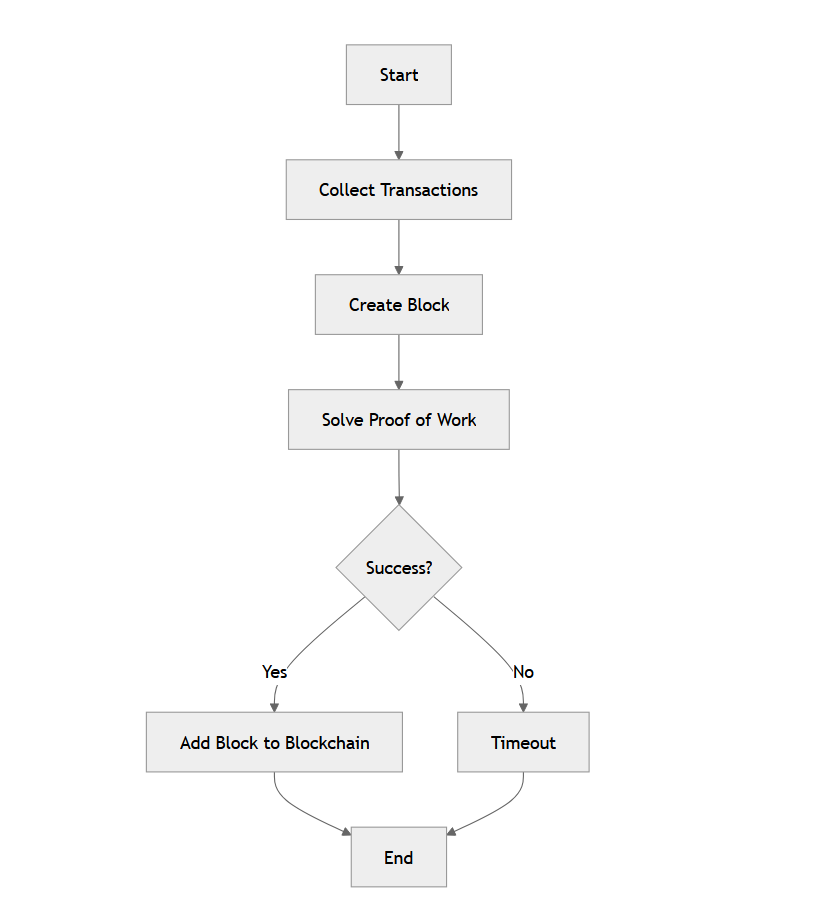
\includegraphics[]{images/5_4_1.PNG}
\begin{verbatim}
Start -> Collect Transactions -> Create Block -> Solve Proof of Work
    -> [Success?] -> Yes -> Add Block to Blockchain -> End
                     No -> Timeout -> End
\end{verbatim}


\subsubsection{Transaction Verification}
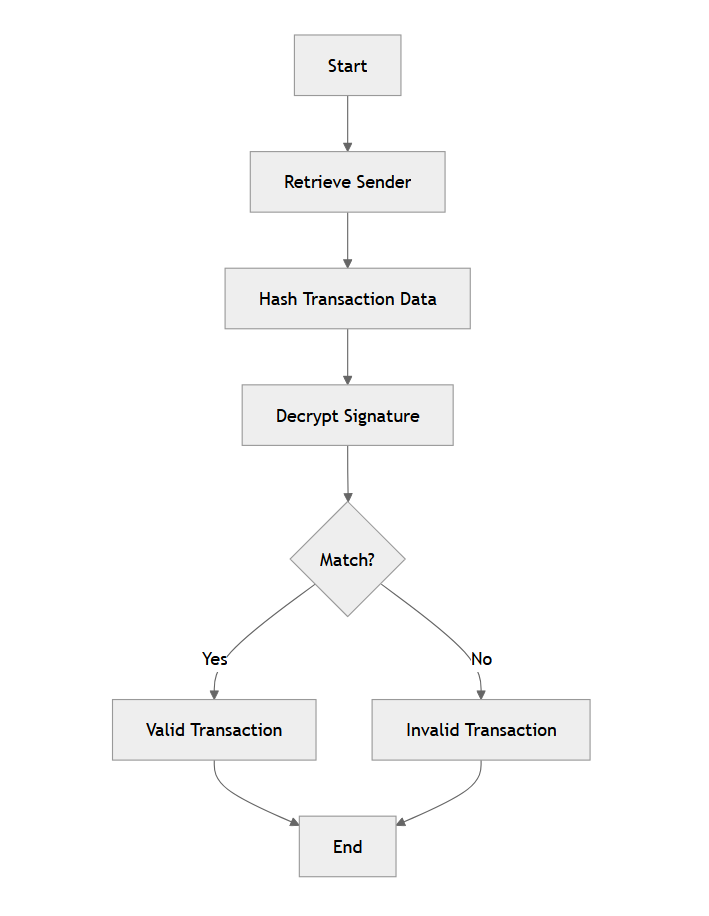
\includegraphics[]{images/5_4_2.PNG}
\begin{verbatim}
Start -> Retrieve Sender -> Hash Transaction Data -> Decrypt Signature
    -> [Match?] -> Yes -> Valid Transaction -> End
                   No -> Invalid Transaction -> End
\end{verbatim}

\subsubsection{Block Verification}
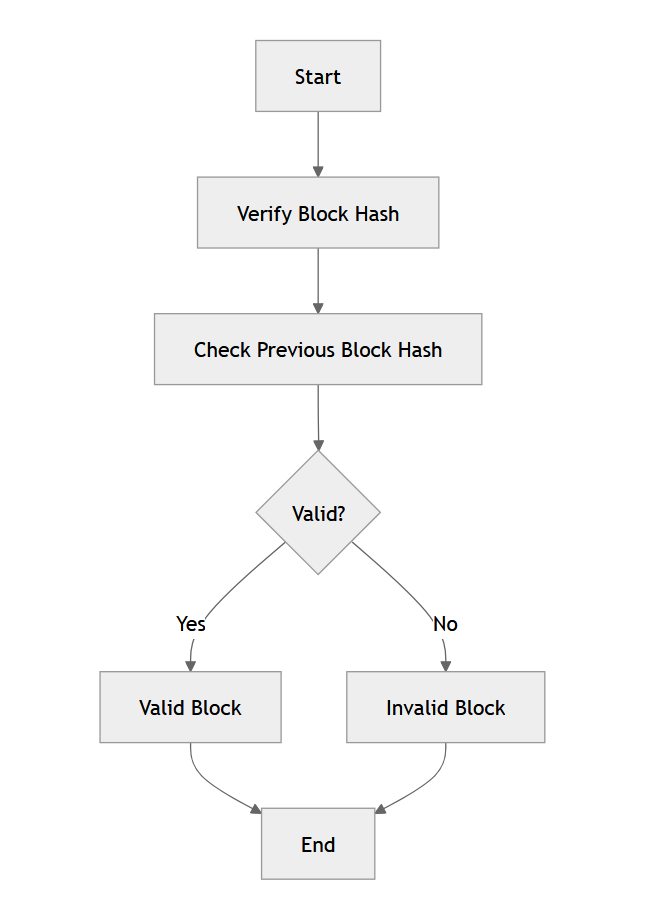
\includegraphics[]{images/5_4_3.PNG}
\begin{verbatim}
Start -> Verify Block Hash -> Check Previous Block Hash
    -> [Valid?] -> Yes -> Valid Block -> End
                   No -> Invalid Block -> End
\end{verbatim}

\subsection{Implementation Details}
\begin{itemize}
    \item \textbf{Cryptography}: RSA is used for digital signatures, and SHA-256 is used for hashing.
    \item \textbf{Singletons}: \texttt{UserManager}, \texttt{MemPool}, and \texttt{BlockChain} are implemented as singletons for centralized management.
    \item \textbf{Timeouts}: Mining has a timeout to prevent infinite loops.
    \item \textbf{Error Handling}: Exceptions are used for invalid operations, such as insufficient funds.
\end{itemize}

This design ensures modularity, security, and scalability for the blockchain system.

\section{Experimental Results}
\subsection{Simulation}
The simulation of the MiniBlockchain system was conducted to validate its core functionalities, including transaction validation, mining, and blockchain verification. Below are the detailed results:

\begin{itemize}
    \item \textbf{Transaction Validation}: Transactions were tested for validity before and after tampering. Initially, valid transactions were successfully verified using the implemented verification mechanism. When transaction details, such as the amount, were altered, the system detected the tampering and flagged the transaction as invalid. This demonstrates the robustness of the digital signature mechanism in ensuring transaction integrity.

    \item \textbf{Mining Process}: The mining process was simulated with multiple transactions in the mempool. Miners successfully collected valid transactions, created new blocks, and solved the proof-of-work puzzle within the specified timeout. The mined blocks were added to the blockchain, and their hashes satisfied the difficulty target. This highlights the effectiveness of the proof-of-work mechanism in maintaining blockchain security.

    \item \textbf{Blockchain Verification}: The entire blockchain was verified to ensure its integrity. Each block's header, transactions, and proof-of-work were validated. The verification process successfully detected tampered blocks and flagged them as invalid. This demonstrates the system's ability to maintain a tamper-proof and consistent blockchain.

    \item \textbf{Merkle Tree Validation}: The Merkle tree was used to verify the integrity of transactions within a block. The generated Merkle root matched the stored Merkle root for valid blocks. When transactions were altered, the Merkle root mismatch was detected, ensuring the integrity of the block's transaction data.

    \item \textbf{Performance Observations}: Mining time increased with the difficulty of the proof-of-work puzzle, as expected. This demonstrates the scalability of the mining process and its ability to adapt to varying difficulty levels. The system efficiently handled multiple transactions and users, showcasing its capability to simulate a realistic blockchain environment.

    \item \textbf{Malicious Actions}: Various malicious actions, such as altering block headers, adding fraudulent transactions, and modifying existing transactions, were simulated. The system successfully detected these actions during the verification process, ensuring the blockchain's security and reliability.
\end{itemize}

These results validate the MiniBlockchain project's implementation of core blockchain functionalities, including transaction validation, mining, and verification. The system effectively ensures data integrity, security, and consistency, making it a reliable educational tool for understanding blockchain technology.

\subsection{Observations}
\begin{itemize}
    \item Mining time increases with the difficulty of proof-of-work.
    \item Tampered transactions are successfully detected and rejected.
\end{itemize}

\section{Conclusion}
The MiniBlockChain project demonstrates the core functionalities of a blockchain system, including transaction validation, mining, and block verification. The system ensures data integrity and security through cryptographic techniques and proof-of-work.

\section{References}
\begin{enumerate}
    \item Java Cryptography Architecture (JCA) Documentation.
    \item Blockchain Basics by Daniel Drescher.
    \item Merkle Tree Concepts in Cryptography.
\end{enumerate}

\section{Appendices}
\subsection{Codebase}
Full source code of the project is available in the \texttt{src/} directory.

\subsection{Simulation Logs}
Output logs from the experimental results are included in the project repository.

\end{document}